\documentclass[12pt,letterpaper]{article}
\usepackage{graphicx,textcomp}
\usepackage{natbib}
\usepackage{setspace}
\usepackage{fullpage}
\usepackage{color}
\usepackage[reqno]{amsmath}
\usepackage{amsthm}
\usepackage{fancyvrb}
\usepackage{amssymb,enumerate}
\usepackage[all]{xy}
\usepackage{endnotes}
\usepackage{lscape}
\newtheorem{com}{Comment}
\usepackage{float}
\usepackage{hyperref}
\newtheorem{lem} {Lemma}
\newtheorem{prop}{Proposition}
\newtheorem{thm}{Theorem}
\newtheorem{defn}{Definition}
\newtheorem{cor}{Corollary}
\newtheorem{obs}{Observation}
\usepackage[compact]{titlesec}
\usepackage{dcolumn}
\usepackage{tikz}
\usetikzlibrary{arrows}
\usepackage{multirow}
\usepackage{xcolor}
\newcolumntype{.}{D{.}{.}{-1}}
\newcolumntype{d}[1]{D{.}{.}{#1}}
\definecolor{light-gray}{gray}{0.65}
\usepackage{url}
\usepackage{listings}
\usepackage{color}

\definecolor{codegreen}{rgb}{0,0.6,0}
\definecolor{codegray}{rgb}{0.5,0.5,0.5}
\definecolor{codepurple}{rgb}{0.58,0,0.82}
\definecolor{backcolour}{rgb}{0.95,0.95,0.92}

\lstdefinestyle{mystyle}{
	backgroundcolor=\color{backcolour},   
	commentstyle=\color{codegreen},
	keywordstyle=\color{magenta},
	numberstyle=\tiny\color{codegray},
	stringstyle=\color{codepurple},
	basicstyle=\footnotesize,
	breakatwhitespace=false,         
	breaklines=true,                 
	captionpos=b,                    
	keepspaces=true,                 
	numbers=left,                    
	numbersep=5pt,                  
	showspaces=false,                
	showstringspaces=false,
	showtabs=false,                  
	tabsize=2
}
\lstset{style=mystyle}
\newcommand{\Sref}[1]{Section~\ref{#1}}
\newtheorem{hyp}{Hypothesis}

\title{Problem Set 1}
\date{Due: October 8, 2026}
\author{Applied Stats/Quant Methods 1}

\begin{document}
	\maketitle
	
	\section*{Instructions}
	\begin{itemize}
	\item Please show your work! You may lose points by simply writing in the answer. If the problem requires you to execute commands in \texttt{R}, please include the code you used to get your answers. Please also include the \texttt{.R} file that contains your code. If you are not sure if work needs to be shown for a particular problem, please ask.
\item Your homework should be submitted electronically on GitHub.
\item This problem set is due before 23:59 on Thursday October 8, 2026. No late assignments will be accepted.
	\end{itemize}
	
	\vspace{1cm}
	\section*{Question 1: Education}

A school counselor was curious about the average of IQ of the students in her school and took a random sample of 25 students' IQ scores. The following is the data set:\\
\vspace{.5cm}

\lstinputlisting[language=R, firstline=36, lastline=36]{PS01_solution_ED.R}  


\vspace{1cm}

\begin{enumerate}
	\item Find a 90\% confidence interval for the average student IQ in the school (As a hint, you first need the mean and SD to create a CI):\\
	
	\ The 90\% confidence interval ranges from 93.95993 to 102.9201. To reach these results, I used the following code:
	
	\lstinputlisting[language=R, firstline=41, lastline=52]{PS01_solution_ED.R}  
	
	\item Next, the school counselor was curious  whether  the average student IQ in her school is higher than the average IQ score (100) among all the schools in the country.\\ 
	
	\noindent Using the same sample, conduct the appropriate hypothesis test with $\alpha=0.05$.
	
	\vspace{1cm}
	
		\ We begin with our assumptions, which specify that our data type is numeric. Our Null Hypothesis H0 states that the sample mean is not higher than the population mean of 100. Our alternative hypothesis H1 states that the sample mean is higher than the population mean of 100. 
	
	\lstinputlisting[language=R, firstline=58, lastline=59]{PS01_solution_ED.R}  
	
	Next we conduct a right tail test and obtain the p-value 0.7215. 
	
	\lstinputlisting[language=R, firstline=60, lastline=65]{PS01_solution_ED.R}  
	
	The p-value is greater than the alpha-level 0.05. Therefore, we we fail to reject the Null hypothesis that the average student IQ at the teacher's school is not higher than the national school average.
	
		\lstinputlisting[language=R, firstline=66, lastline=66]{PS01_solution_ED.R}
	
\end{enumerate}

\newpage

	\section*{Question 2: Political Economy}

\noindent Researchers are curious about what affects the amount of money communities spend on addressing homelessness. The following variables constitute our data set about social welfare expenditures in the USA. \\
\vspace{.5cm}


\begin{tabular}{r|l}
	\texttt{State} &\emph{50 states in US} \\
	\texttt{Y} & \emph{per capita expenditure on shelters/housing assistance in state}\\
	\texttt{X1} &\emph{per capita personal income in state} \\
	\texttt{X2} &  \emph{Number of residents per 100,000 that are "financially insecure" in state}\\
	\texttt{X3} &  \emph{Number of people per thousand residing in urban areas in state} \\
	\texttt{Region} &  \emph{1=Northeast, 2= North Central, 3= South, 4=West} \\
\end{tabular}

\vspace{.5cm}
\noindent Explore the \texttt{expenditure} data set and import data into \texttt{R}.
\vspace{.5cm}
\lstinputlisting[language=R, firstline=71, lastline=71]{PS01_solution_ED.R}  
\vspace{.5cm}
\begin{itemize}

\item
Please plot the relationships among \emph{Y}, \emph{X1}, \emph{X2}, and \emph{X3}? What are the correlations among them (you just need to describe the graph and the relationships among them)?

\vspace{.5cm}

\ I plot the relationships among Y, X1, X2, and X3 for an overview using a bubble chart as follows: 
\vspace{.5cm}
	\lstinputlisting[language=R, firstline=77, lastline=86]{PS01_solution_ED.R}
	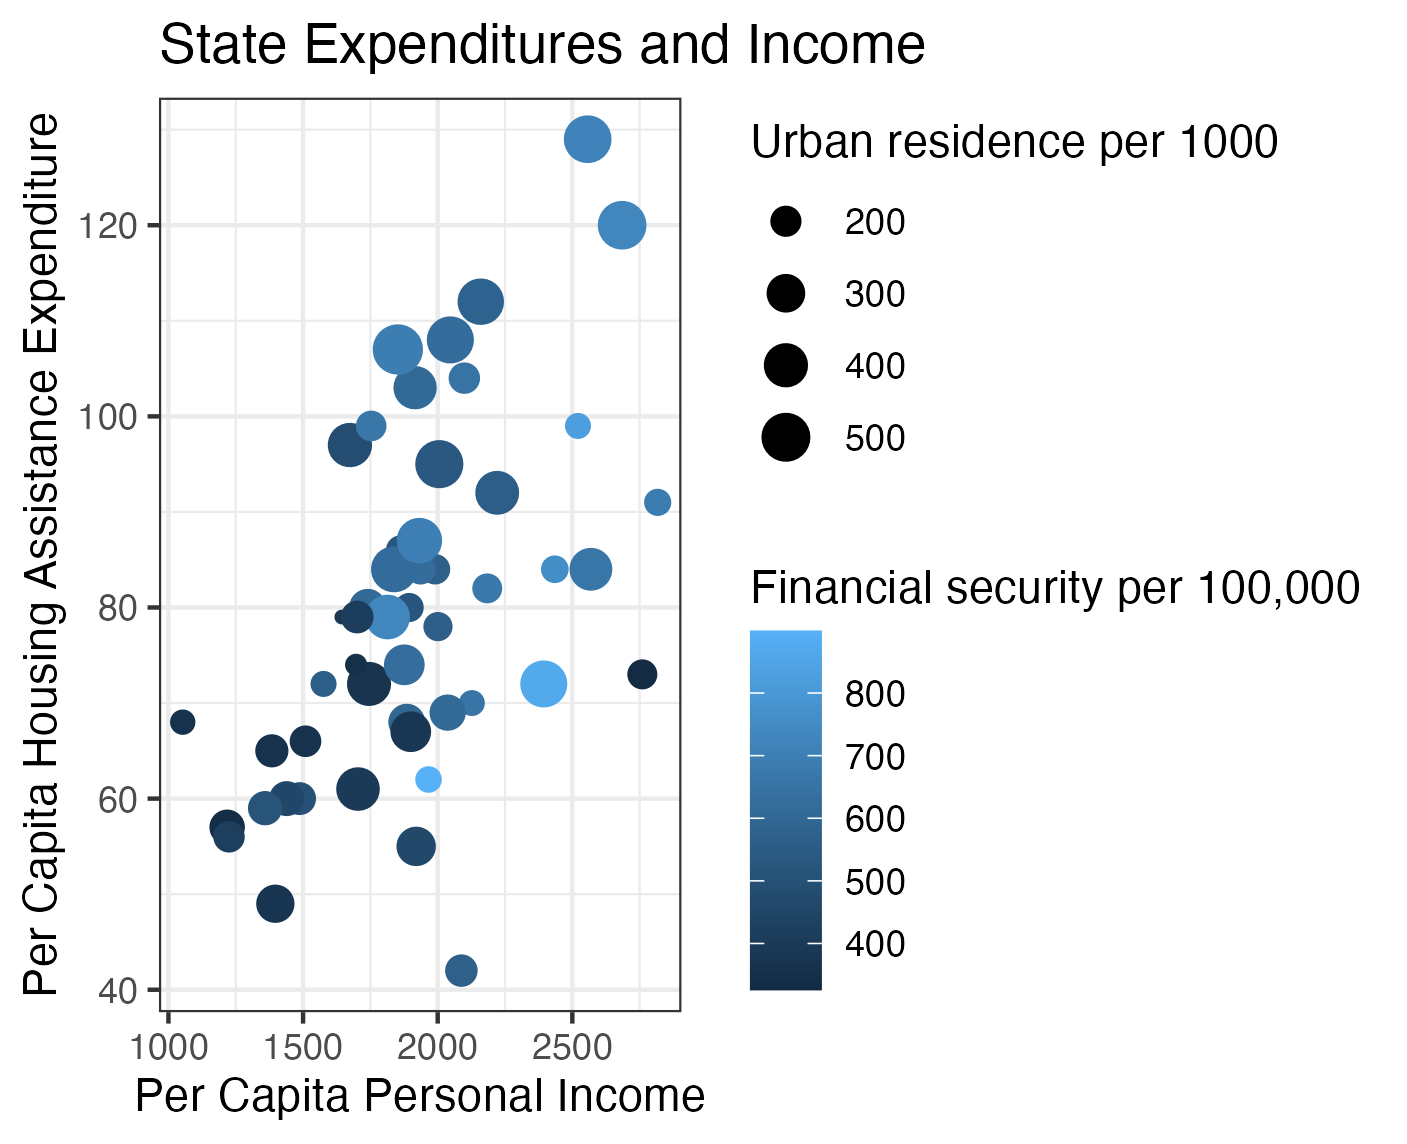
\includegraphics{PS01plot1.png}
	\vspace{.5cm}
	
	From this chart, it appears there is an association between a higher per capita expenditure for housing assistance and a higher income.
	
	To closer examine the other relationships, I then plot each relationship in a scatterplot separately: 
	
	\vspace{.5cm}
	
	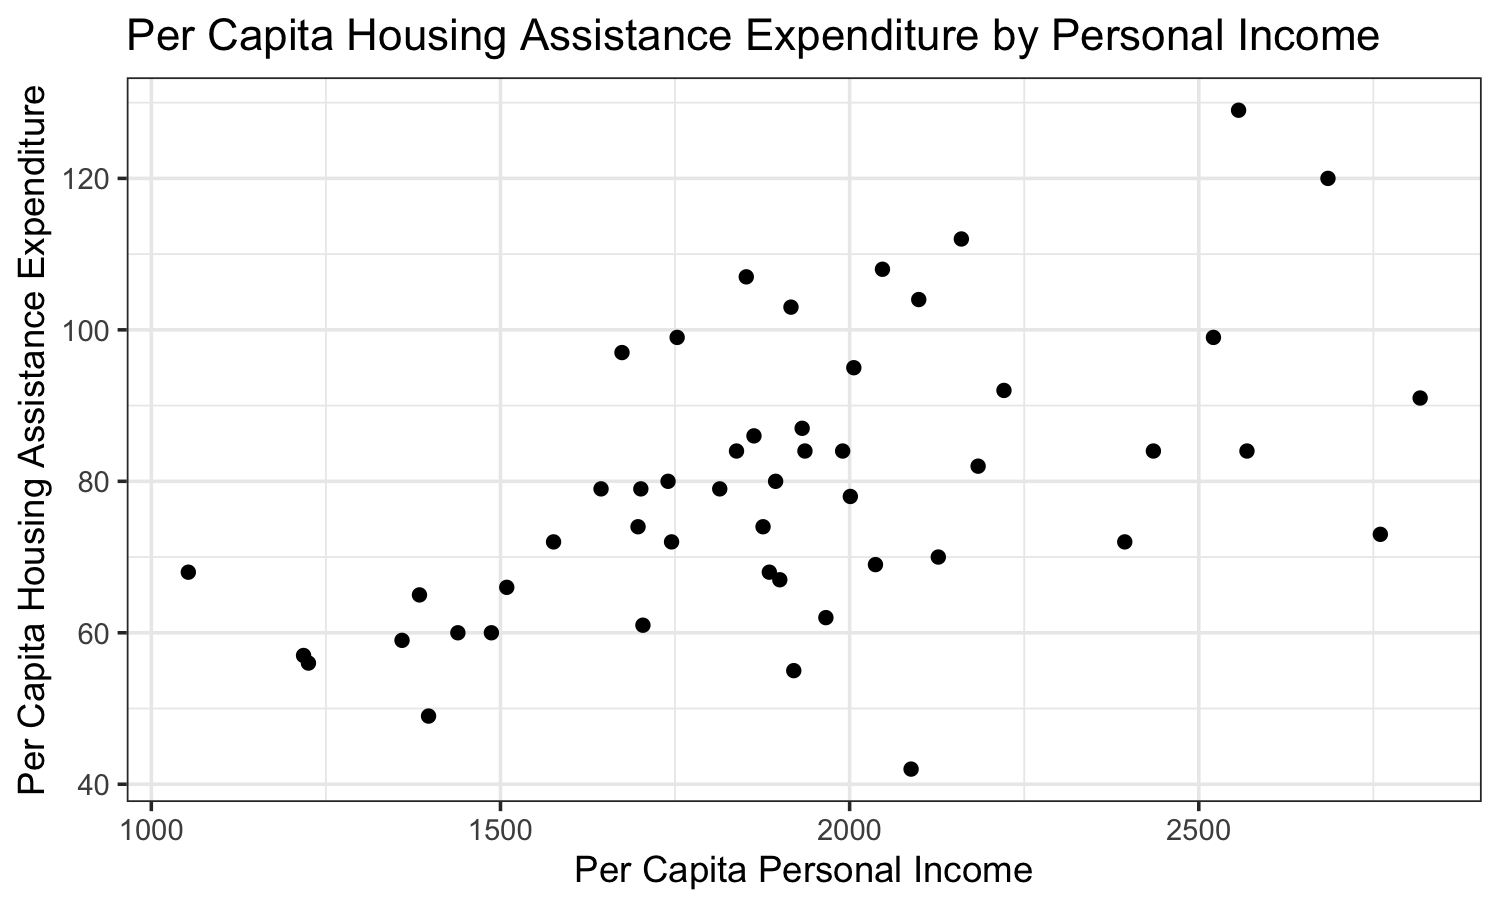
\includegraphics[width=.9\linewidth,height=.25\textheight,keepaspectratio]{plot1.png}
\vspace{.5cm}

The scatterplot implies a positive linear association between per capita housing assistance expenditure and per capita personal income in the states.
\vspace{.5cm}

	\lstinputlisting[language=R, firstline=89, lastline=96]{PS01_solution_ED.R}
	
	Each plot is generated by the above code, with labels and variables exchanged as needed. The rest of the relationships are plotted below without replicating the code.
	
	\vspace{.5cm}
	
	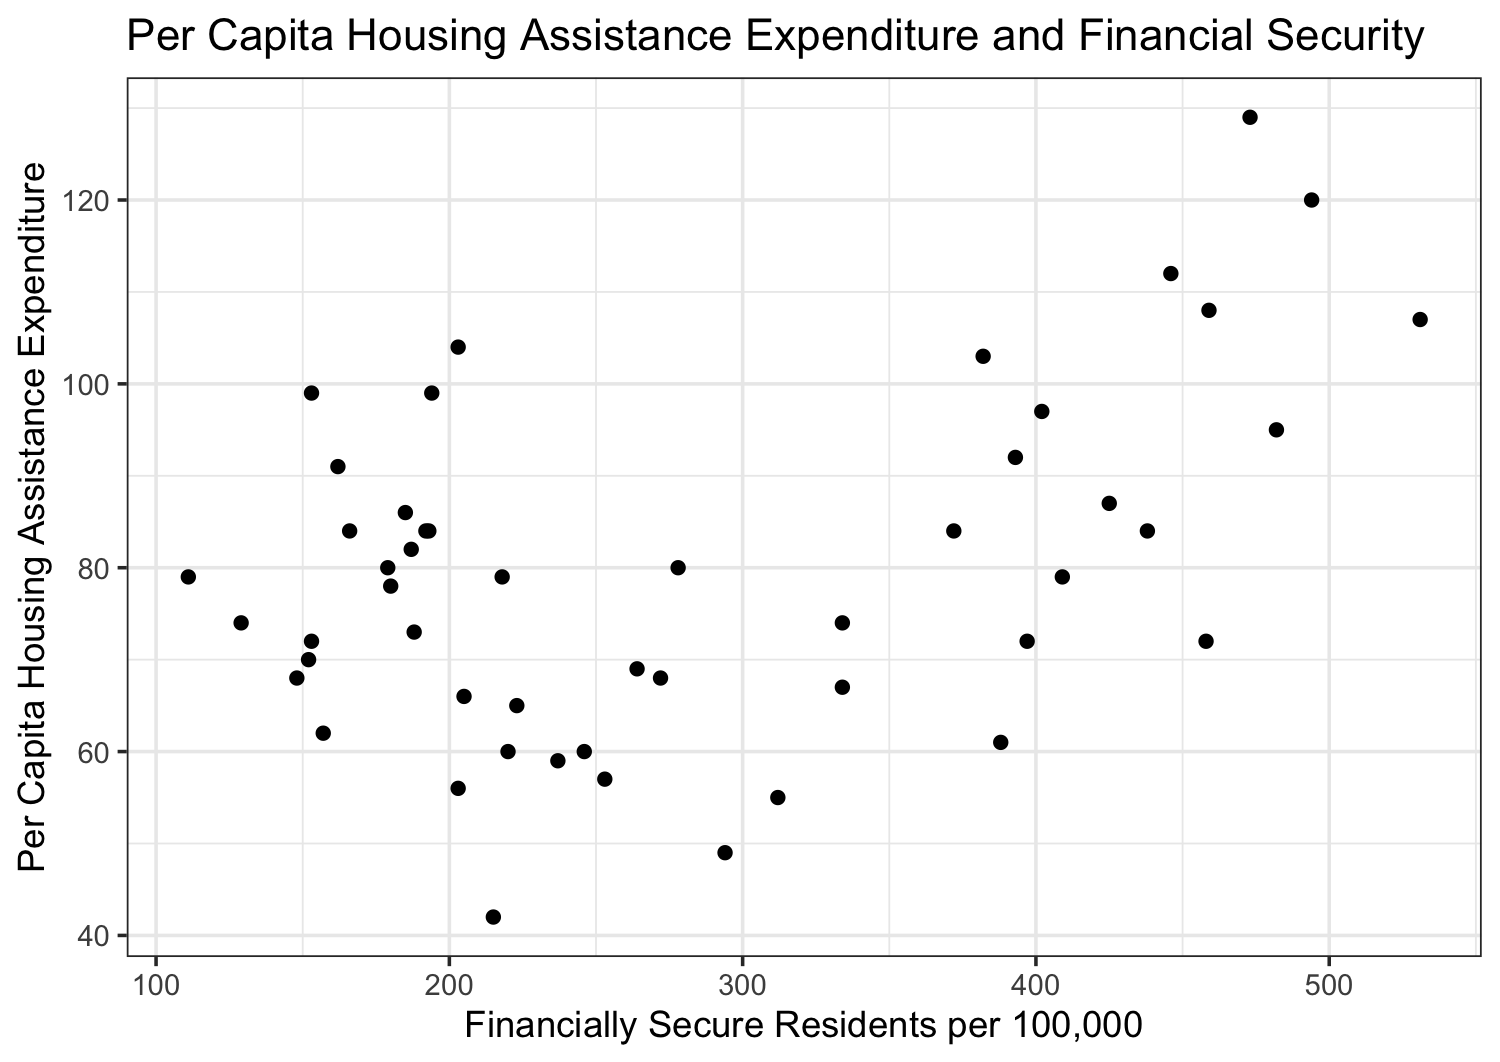
\includegraphics[width=.9\linewidth,height=.25\textheight,keepaspectratio]{plot2.png}
	
		\vspace{.5cm}
		
		The scatterplot shows a slightly U-shaped distribution, showing more housing assistance expenditure in areas with financially stable residents <200 and >400 per 100,000.
		
		\vspace{.5cm}
		
	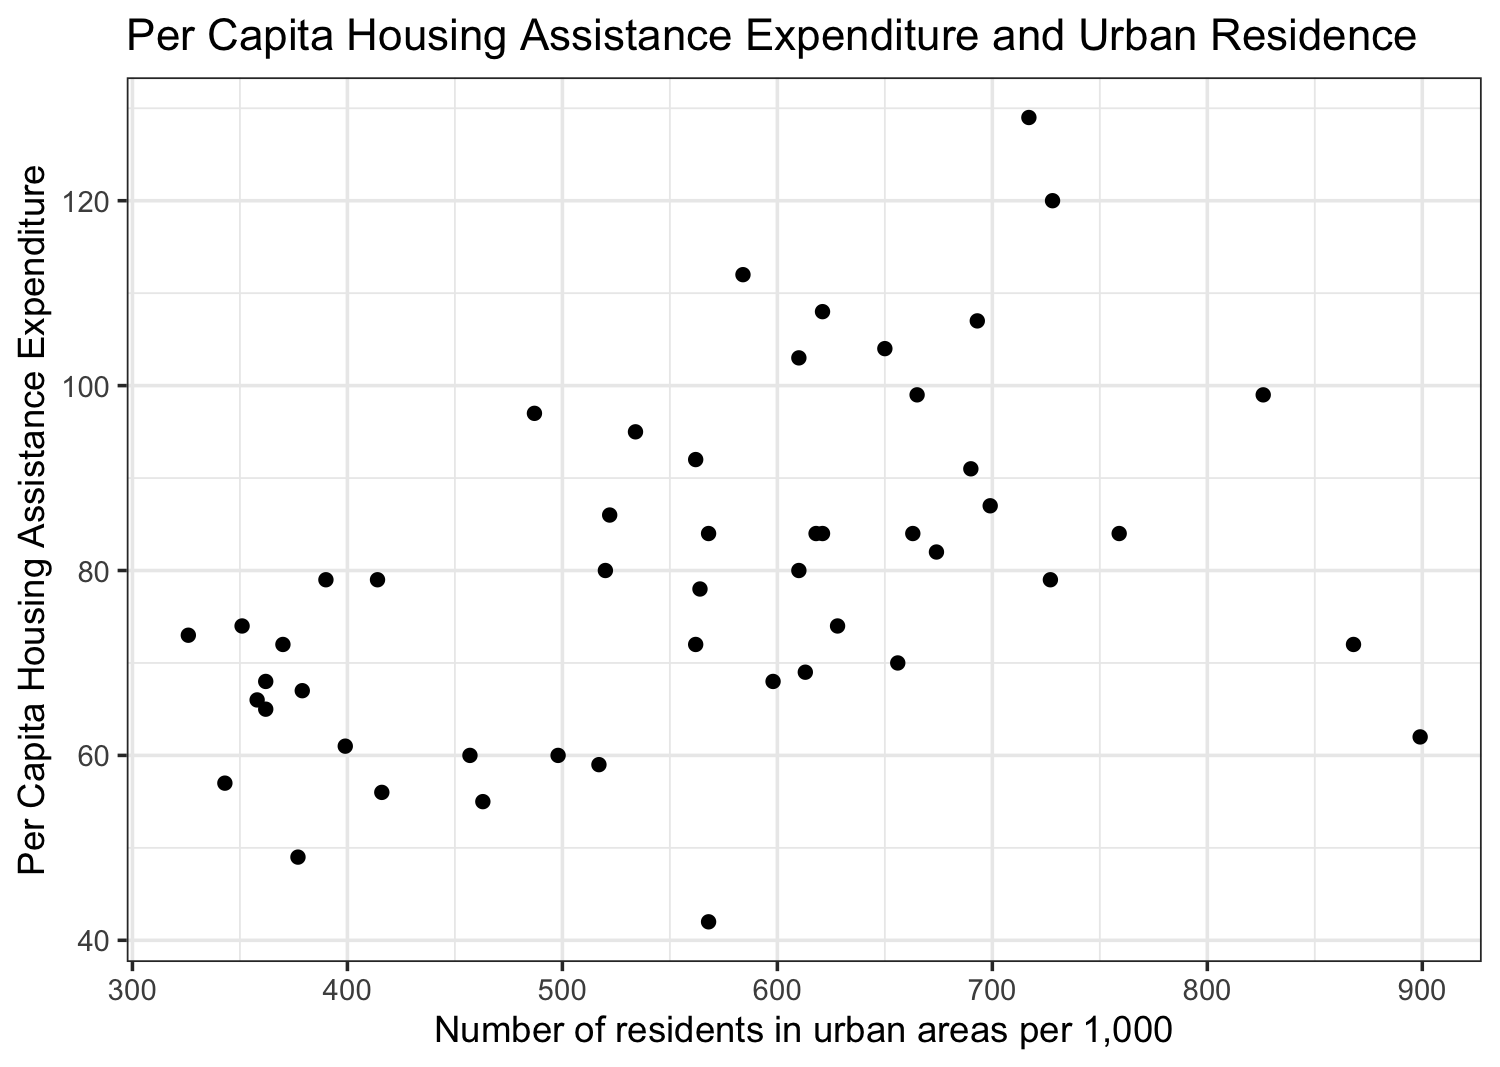
\includegraphics[width=.9\linewidth,height=.25\textheight,keepaspectratio]{plot3.png}
			
		\vspace{.5cm}
		
		The scatterplot shows a positive linear distribution of the number of urban area residents and the per capita ousing assistance expenditure.
		
		\vspace{.5cm}
			
	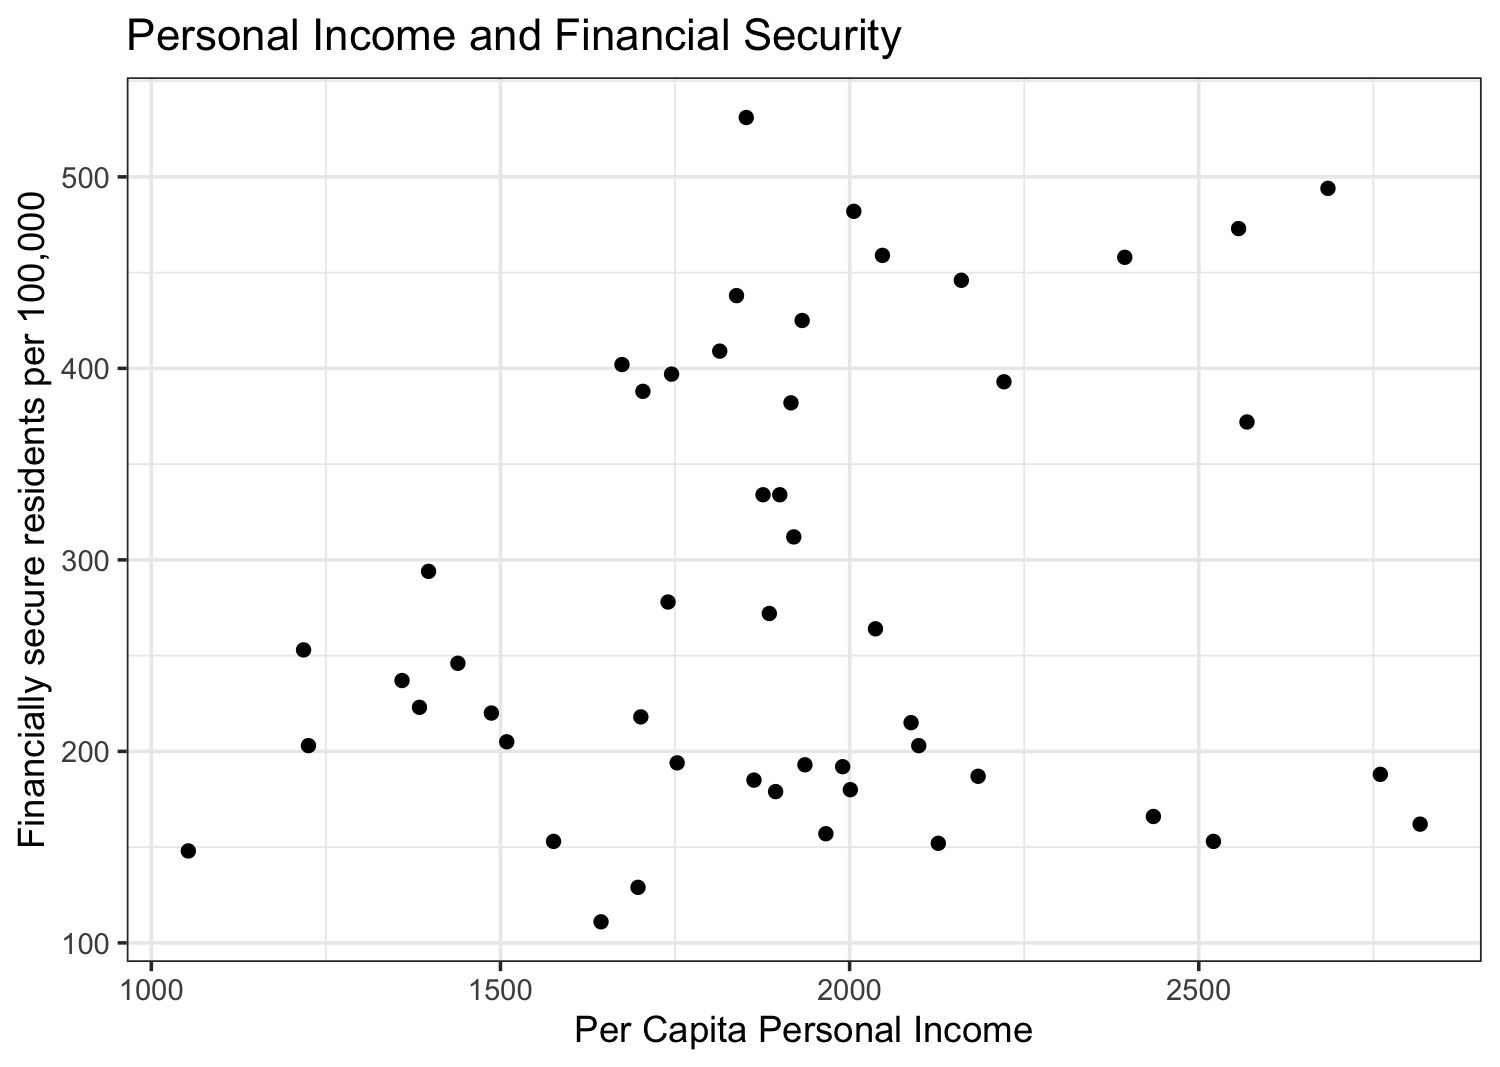
\includegraphics[width=.9\linewidth,height=.25\textheight,keepaspectratio]{plot4.png}
	
		\vspace{.5cm}
		
		The scatterplot shows no association between per capita personal income and financially secure residents per 100,000.
		
		\vspace{.5cm}
				
	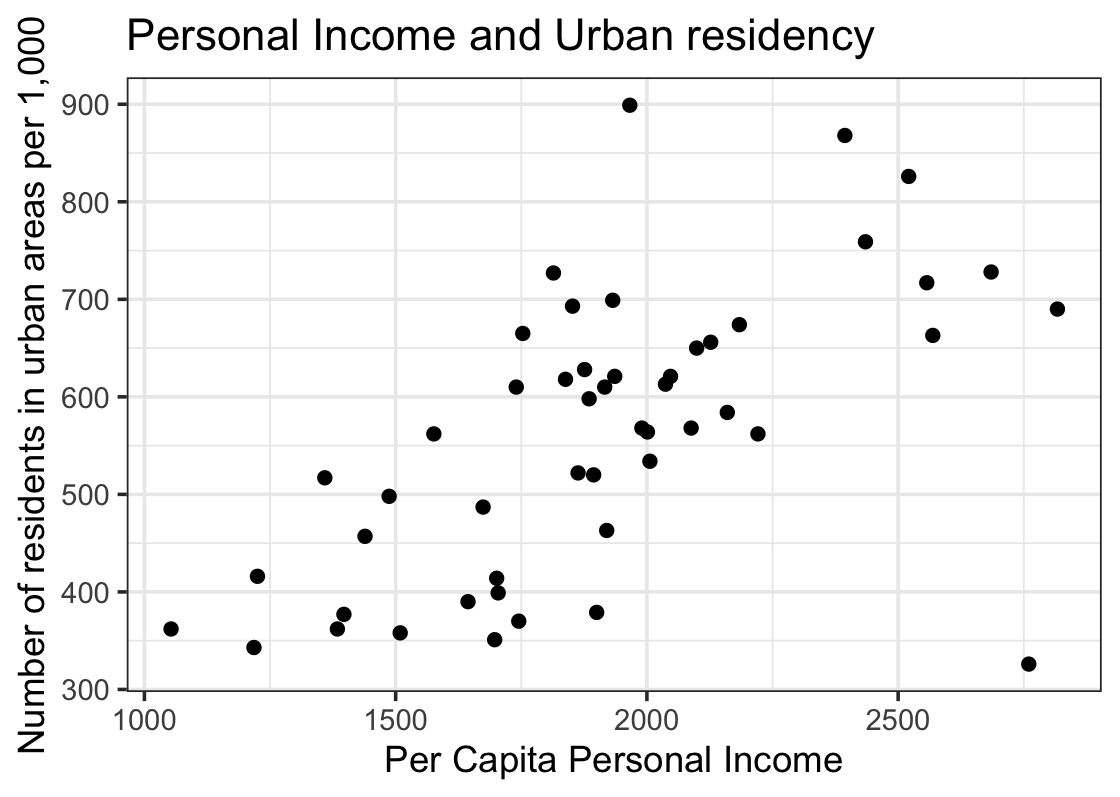
\includegraphics[width=.9\linewidth,height=.25\textheight,keepaspectratio]{plot5.png}
	
		\vspace{.5cm}
		
		The scatterplot shows a positive linear association between per capita personal income and the number of residents in urban areas per 1,000.
		
		\vspace{.5cm}
					
					
	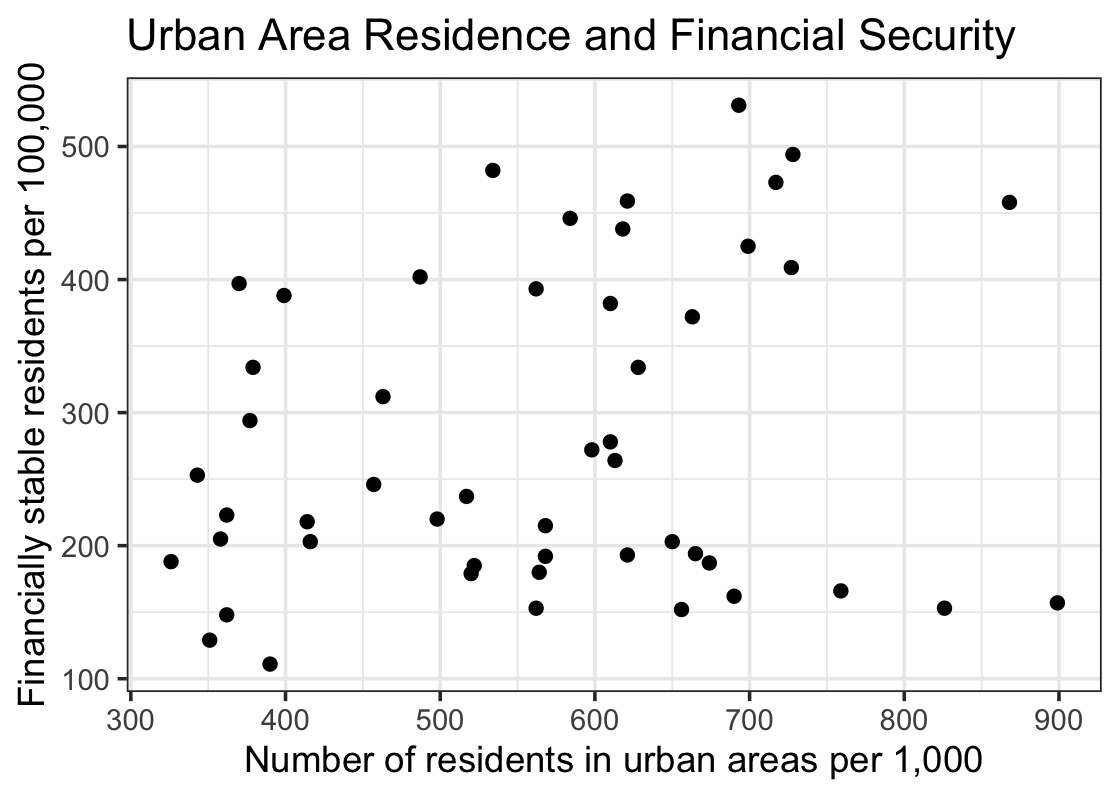
\includegraphics[width=.9\linewidth,height=.25\textheight,keepaspectratio]{plot6.png}
	
		\vspace{.5cm}
		
		The scatterplot shows no association between the number of urban area residents per 1,000 and the number of financially stable residents per 100,000.
		
		\vspace{.5cm}
						
\vspace{.5cm}
\item
Please plot the relationship between \emph{Y} and \emph{Region}? On average, which region has the highest per capita expenditure on housing assistance?
\vspace{.5cm}


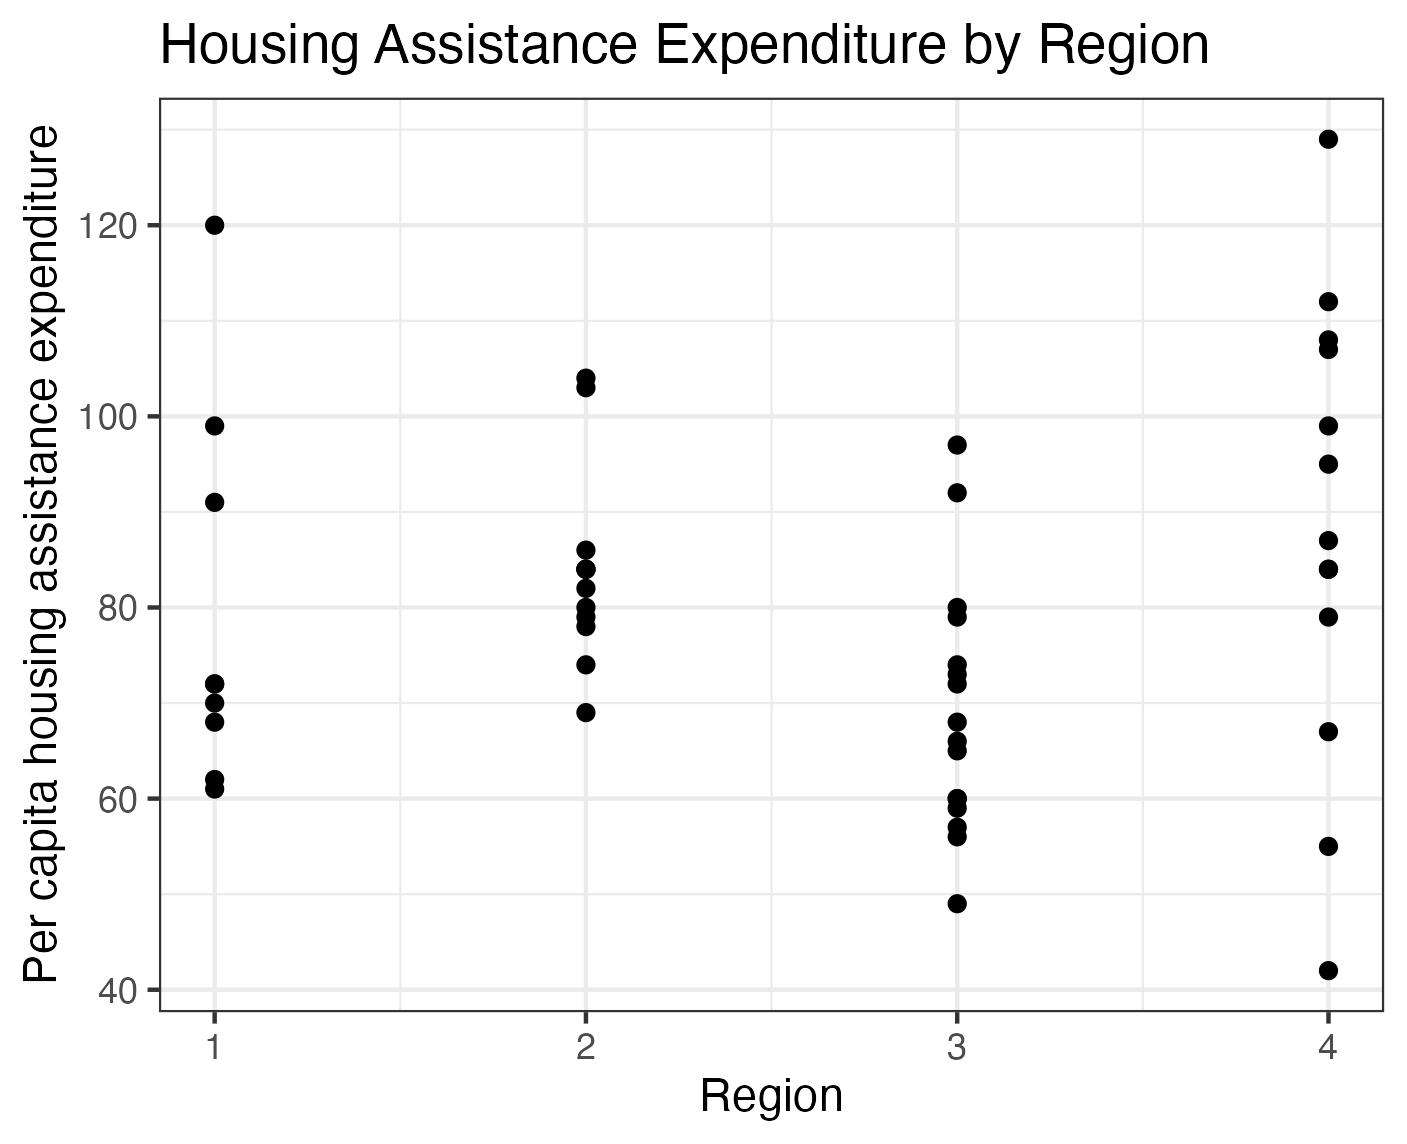
\includegraphics[width=.9\linewidth,height=.25\textheight,keepaspectratio]{PS01plot2.png}

\vspace{.5cm}

On average, the Western region has the highest per capita housing assistance expenditure. 

\vspace{.5cm}

In the code below, I have first transformed the Regions into factors in order to allow for later shape adjustment and to change their names in the graph for clarity.

\vspace{.5cm}

	\lstinputlisting[language=R, firstline=155, lastline=165]{PS01_solution_ED.R}



\item
Please plot the relationship between \emph{Y} and \emph{X1}? Describe this graph and the relationship. Reproduce the above graph including one more variable \emph{Region} and display different regions with different types of symbols and colors.

		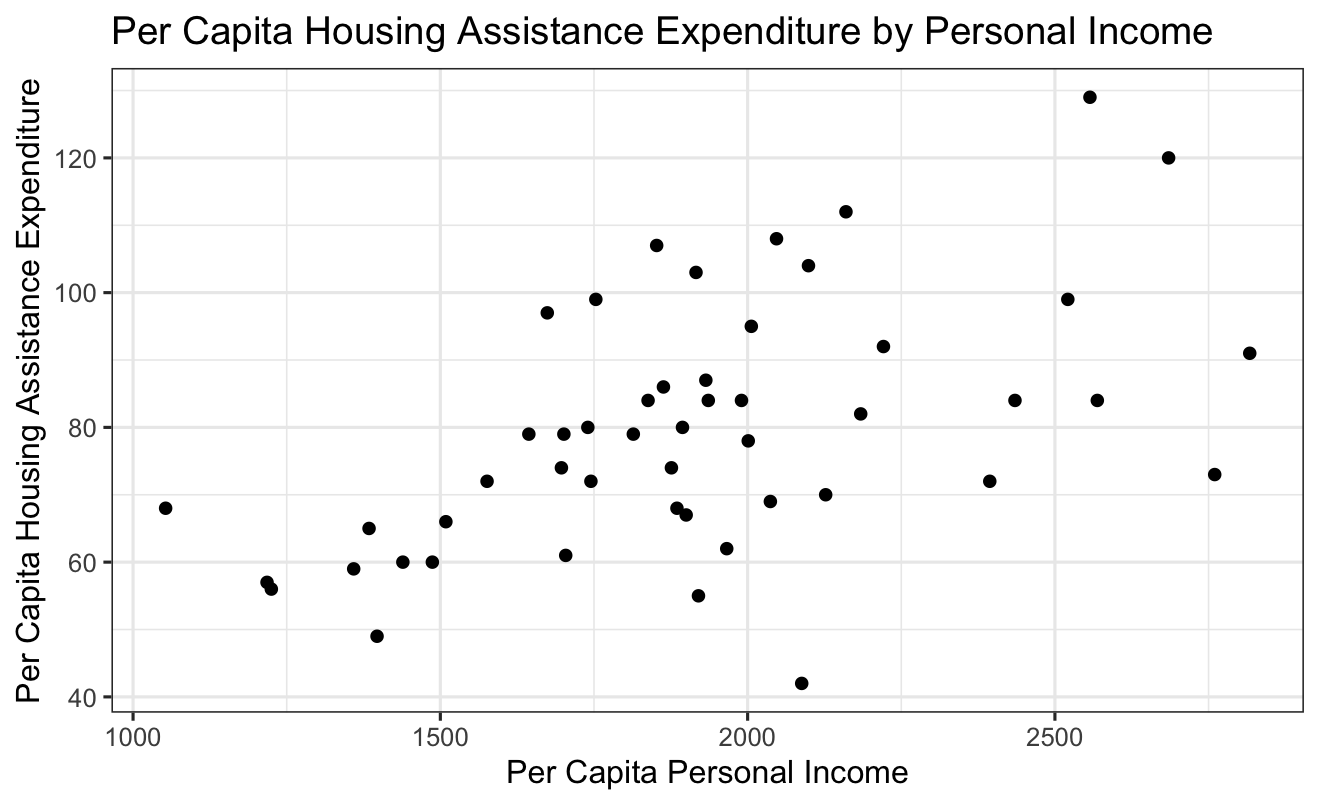
\includegraphics[width=.9\linewidth,height=.25\textheight,keepaspectratio]{PS01plot3.png}
		
		\vspace{.5cm}
		
		The above plot shows that housing assistance expenditure is highest on average in states with a personal income around the 2000 mark.
		
		\vspace{.5cm}
		
		Here the corresponding code:
		
			\vspace{.5cm}
		
	\lstinputlisting[language=R, firstline=171, lastline=177]{PS01_solution_ED.R}
	
	Below is the same graph with Regions added in. 
	
	\vspace{.5cm}
	
	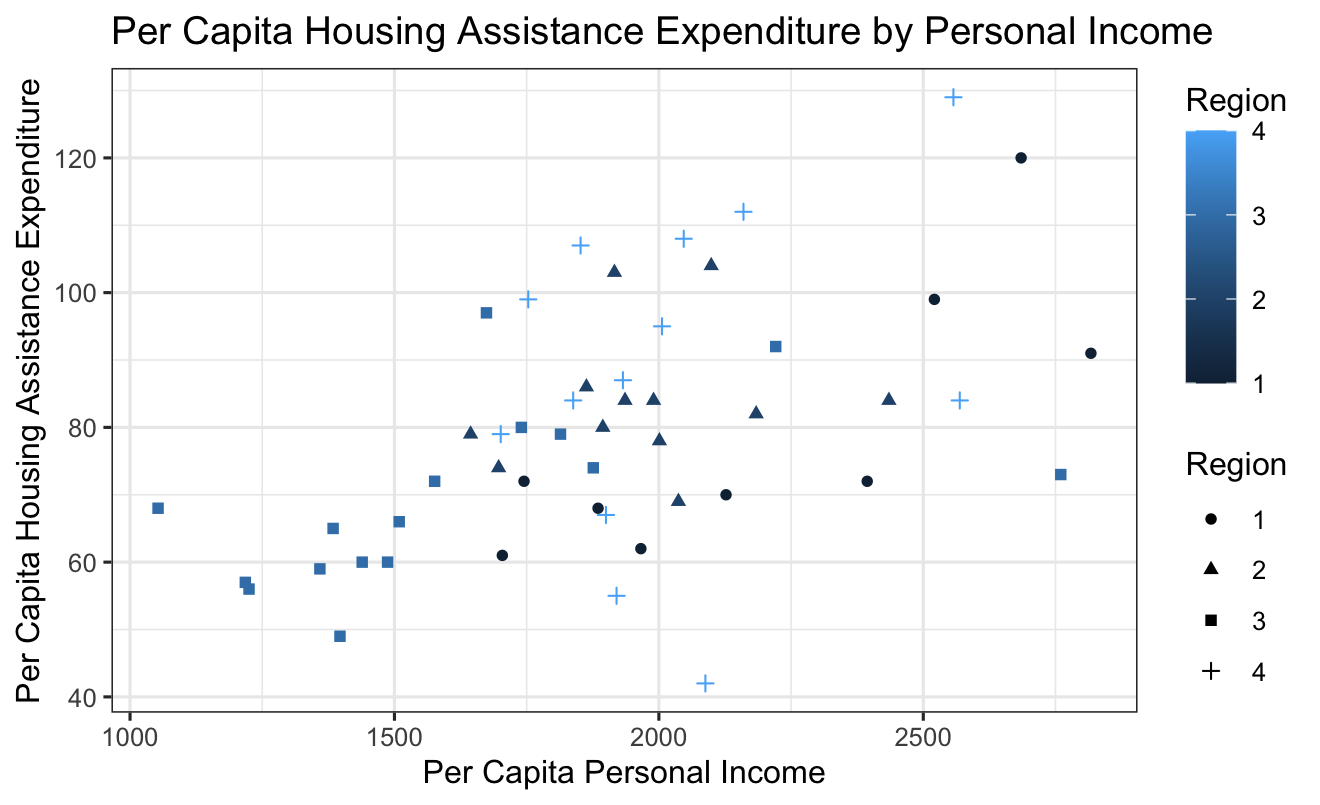
\includegraphics[width=.9\linewidth,height=.25\textheight,keepaspectratio]{PS01plot4.png}
	
	\vspace{.5cm}
	
	\lstinputlisting[language=R, firstline=181, lastline=191]{PS01_solution_ED.R}
\end{itemize}


\end{document}
